%% PNAStwoS.tex

%% BASIC CLASS FILE
\documentclass{pnastwo2}

%% ADDITIONAL OPTIONAL STYLE FILES
\usepackage{graphicx}
%\usepackage{pnastwoF}
\usepackage{amssymb,amsfonts,amsmath}
\usepackage{caption}
\usepackage{subcaption}
\usepackage{float}
\usepackage{wrapfig}
\usepackage{caption}
%% OPTIONAL MACRO DEFINITIONS
\def\s{\sigma}

%%%%%%%%%%%%
\url{http://cs230.stanford.edu/}
\copyrightyear{2019}
\issuedate{CS 230}
\volume{Winter 2019}
%%%%%%%%%%%%

\begin{document}

\title{Making yourself into a work of art}

\author{Kiah Hardcastle \affil{1}{Neurosciences Program, Stanford University},
\and Julie Makelberge\affil{2}{Graduate School of Business, Stanford University}}

\contributor{Project Milestone for CS 230: Deep Learning, February 2019}

\maketitle

\begin{article}

\begin{abstract}

Here we begin the implementation of a deep learning framework that will swap the face in an artistic painting with the face in a separate image. For example, given a headshot and a picture of the Mona Lisa, this framework would inpaint the headshot face into the face of the Mona Lisa, while retaining the artistic style of the Mona Lisa. Completion of this project requires several steps: identifying the face in both images, excising the particular face region, aligning the face features in both images by finding a dense correspondence between the two images, generating a new image that blends the two by performing visual attribute transfer between the two images, and the finally replacing the previously excised region in the artistic image with the newly generated image.

\end{abstract}

\dropcap{S}wapping faces between images ... add some introduction here.

\section{Methods}
\subsection{Data collection and pre-processing}

Fortunately, as we are using methods of neural style transfer, or similar to neural style transfer, using VGG-19 networks pre-trained on ImageNet, we do not need large numbers of new images with which to train our network. However, there are large datasets of artwork and faces available on the internet, which we plan to take advantage of here in order to demonstrate our approach. To generate our dataset of artwork, we will use the Web Gallery of Art. This dataset is free to use for educational purposes and contains the meta data and links to images for more than 45,000 works of art, 31,000 of which are paintings. In order to create the dataset, we wrote write a script to download these images (code is attached at the end of this document). To generate a dataset of faces, we will either use our own headshots (an example is included in this report), or images downloaded from the celebA dataset (http://mmlab.ie.cuhk.edu.hk/projects/CelebA.html). 

\begin{figure}
	\begin{center}
		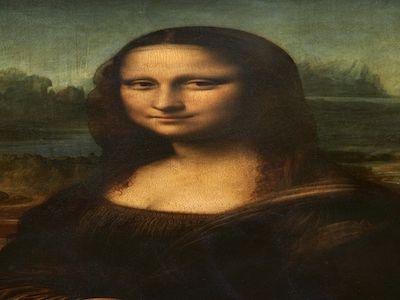
\includegraphics[width=.3\textwidth]{mona_lisa.jpg}
		\caption{{\bfseries A}. Example of artistic image containing a face (the Mona Lisa).} \label{fig:mona}
	\end{center}
\end{figure} 

\begin{figure}
	\begin{center}
		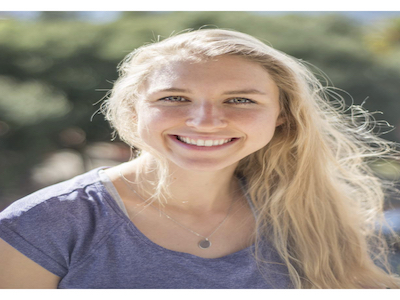
\includegraphics[width=.3\textwidth]{headshot_kiahhardcastle}
		\caption{{\bfseries A}. Example of other image containing a face (a headshot of Kiah Hardcastle).} \label{fig:kiah}
	\end{center}
\end{figure} 

\subsection{Model architecture}

As mentioned above, successful completion of our task requires several intermediate steps. First, assuming that the images containing faces are not simply headshots that are perfectly aligned with each other, we must identify the region containing the face in both images (art image = image A with face A, other image = image B with face B). In order to do this, we will use a face recognition algorithm (XXX) that will return the bounding box of the face. This method will then return to us two semantically similar images - an image of a face - with which we can then use in the rest of our pipeline.

Second, we will then follow the procedure outlined in the paper "Visual Attribute Transfer through Deep Image Analogy", by Jing Liao et al. Briefly, .... 

Third, once we have generated a new image C that contains face C (the face in B, but in the style of face A), we must then replace the region around face A in image A (what was originally excised) with the new image C. It may be the case that additional smoothing, or matching of the original image will have to take place in order to smooth the boundaries between image C and the region around face A. 

To get a sense of the data and the problem at hand, we performed neural style transfer on images that were already roughly matched in terms of semantic similarity. Images A (see Figure 1) and B (see Figure 2) were chosen so that faces in both images were quite prominent, and were in similar positions. Specifically, following the Neural Style Transfer code in the coursera course, we used the pre-trained weights from the VGG-19 network trained on ImageNet. We then used activations from layers within the network to generate content activations from image B, and style activations from image A. 

\section{Results}

\subsection{Output of model}

\begin{figure}
	\begin{center}
		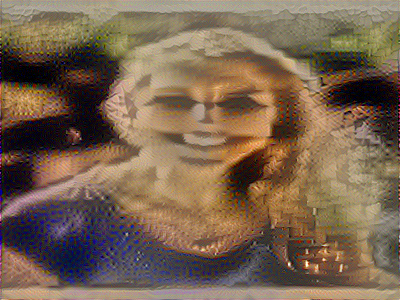
\includegraphics[width=.3\textwidth]{nst.png}
		\caption{{\bfseries A}. Output of neural style transfer between images in Fig 1 and 2} \label{fig:nst}
	\end{center}
\end{figure} 

\subsection{Model performance evaluation}

As described above, our algorithm will return new images. One method of evaluation is qualitative analysis - i.e. determining by eye whether the face was successfully swapped within the piece of art. In order to quantify this more precisely, we plan to conduct polls of groups of people (~100) to determine if they believe the generated image looks like the original image with a face swap. Additionally, we may implement a more rigorous method, in which we attempt to detect the original face in the artistic painting via face verification. The performance of the face verification model could then serve as a proxy for how well the face from the non-art image was inpainted.

\section{Summary}

In summary, thus far we have applied neural style transfer to generate a new image that contains the style of an artwork piece, using the content of the headshot. This is a first step in our procedure, and while it does not perform very well, this allowed us to gain an understanding of the challenges in pre-processing data while allowing understanding the limitations of neural style transfer alone. 


\begin{acknowledgments}
We thank Andrew Ng and Kian Katanforoosh for teaching us the techniques used in this project, and to our project TA Kaidi Cao for guiding us towards workable solutions for our problem and pointing us to relevant literature.
\end{acknowledgments}




\end{article}
\end{document}